\section{Two Dimensions}
Let 
\begin{equation}
\mbf{y} = A\mbf{x} + \mbf{n},
\end{equation}
where 
\begin{align}
x &\in \brak{\mbf{s}_0,\mbf{s}_1}, 
\mbf{s}_0 = 
\begin{pmatrix}
1 
\\
0
\end{pmatrix},
\mbf{s}_1 = 
\begin{pmatrix}
0 
\\
1
\end{pmatrix}
\\
\mbf{n} &= 
\begin{pmatrix}
n_1
\\
n_2
\end{pmatrix},
n_1,n_2 \sim \gauss{0}{1}.
\end{align}
%
\begin{enumerate}
%%
\item
\label{ch5_fsk}
Plot 
%
\begin{equation}
\mbf{y}|\mbf{s}_0 \text{ and } \mbf{y}|\mbf{s}_1
\end{equation}
%
on the same graph using a scatter plot.\\
\solution Refer \figref{fig:biv_scatter} for plot,
\begin{lstlisting}
chapter5/codes/biv_scatter.py
\end{lstlisting}
%
\begin{figure}[H]
\centering
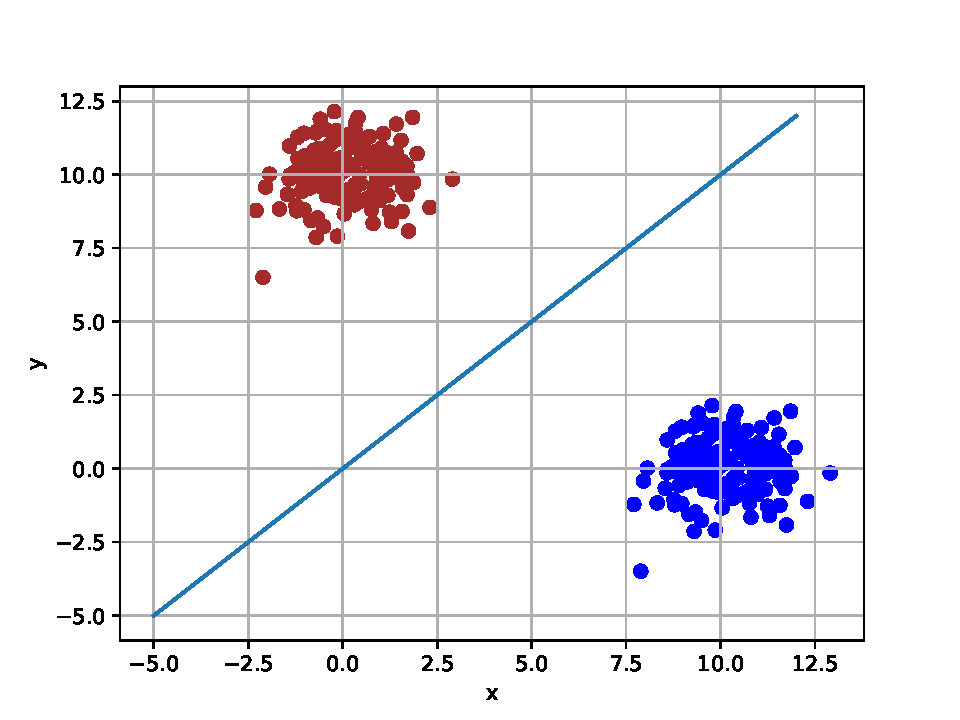
\includegraphics[scale=0.8]{chapter5/figs/biv_scatter.pdf}
\caption{Scatter plot of $\mbf{y}|\mbf{s}_0$ and $\mbf{y}|\mbf{s}_1$ }
\label{fig:biv_scatter}
\end{figure}

%
\item
For the above problem, find a decision rule for detecting the symbols $\mbf{s}_0 $ and $\mbf{s}_1$.\\
%\solution The multivariate Gaussian distribution is defined as
%
%\begin{multline}
%\label{eq:multivariate}
%p_{\mathbf{y}}(y_1,\dots,y_k)
%\\
%=\frac{1}{\sqrt{\brak{2\pi}^k\abs{\bm{\sigma}}}}\exp\cbrak{-\frac{1}{2}\brak{\mathbf{y}-\bm{\mu}}^T\bm{\sigma}^{-1}\brak{\mathbf{y}-\bm{\mu}}}
%\end{multline}
%%
%where $\bm{\mu}$ is the mean vector, $\bm{\sigma} = E\sbrak{\brak{\mathbf{x}-\bm{\mu}}\brak{\mathbf{x}-\bm{\mu}}^T}$ is the covariance matrix and $\abs{\bm{\sigma}}$ is the determinant of $\bm{\Sigma}$.
%\begin{multline}
%\label{eq:multivariate}
%p_{\mathbf{y}}(y_1,y_2)
%\\
%=\frac{1}{2\pi\sqrt{\abs{\bm{\sigma}}}}\exp\cbrak{-\frac{1}{2}\brak{\mathbf{y}-\bm{\mu}}^T\bm{\sigma}^{-1}\brak{\mathbf{y}-\bm{\mu}}}
%\end{multline}
%\begin{multline}
%p\brak{\vec{y}|s_0}
%\\
%=\frac{1}{2\pi\sqrt{\abs{\bm{\sigma}}}}\exp\cbrak{-\frac{1}{2}\brak{\mathbf{y}-\bm{s_0}}^T\bm{\sigma}^{-1}\brak{\mathbf{y}-\bm{s_0}}}
%\label{eq:multivariate1}
%\end{multline}
%\begin{multline}
%p\brak{\vec{y}|s_1}
%\\
%=\frac{1}{2\pi\sqrt{\abs{\bm{\sigma}}}}\exp\cbrak{-\frac{1}{2}\brak{\mathbf{y}-\bm{s_1}}^T\bm{\sigma}^{-1}\brak{\mathbf{y}-\bm{s_1}}}
%\label{eq:multivariate2}
%\end{multline}
%According to the MAP criterion, assuming equiprobably symbols,optimal decison criteria can be found by equating \eqref{eq:multivariate1},\eqref{eq:multivariate2}
%\begin{equation}
%p\brak{\vec{y}|s_0}=p\brak{\vec{y}|s_1}
%\label{eq:map_bfsk_dec1}
%\end{equation}
%\begin{multline*}
%\frac{1}{2\pi\sqrt{\abs{\bm{\sigma}}}}\exp\cbrak{-\frac{1}{2}\brak{\mathbf{y}-\bm{s_0}}^T\bm{\sigma}^{-1}\brak{\mathbf{y}-\bm{s_0}}} \\ =\frac{1}{2\pi\sqrt{\abs{\bm{\sigma}}}}\exp\cbrak{-\frac{1}{2}\brak{\mathbf{y}-\bm{s_0}}^T\bm{\sigma}^{-1}\brak{\mathbf{y}-\bm{s_0}}}
%\end{multline*}
%\begin{align*}
%\brak{\vec{y}-\vec{s}_0}^\top \brak{\vec{y}-\vec{s}_0} &= \brak{\vec{y}-\vec{s}_1}^\top \brak{\vec{y}-\vec{s}_1}\\
%\vec{y}^\top\vec{y} - 2\vec{s}_0^\top \vec{y} + \vec{s}_0^T\vec{s}_0 &= \vec{y}^\top\vec{y} - 2\vec{s}_1^\top \vec{y} + \vec{s}_1^T\vec{s}_1\\
% 2\brak{\vec{s}_1-\vec{s}_0}^\top \vec{y} &= \norm{\vec{s}_1}^2 - \norm{\vec{s}_0}^2\\
%\brak{\vec{s}_1-\vec{s}_0}^\top \vec{y} &= 0\\
%\myvec{-1\\1}^\top \vec{y} &= 0
%\end{align*}



\solution
The real vector  \begin{align}
s_0 =(s_1,\dots,s_n)^\top \\
s_1 =(s_1,\dots,s_n)^\top \\
\end{align}
For the given $s_0$, $n_1,n_2 \sim \gauss{0}{1}$.
\begin{align}
p\brak{\vec{y}|s_0}=\frac{1}{\sqrt{\brak{2\pi\sigma^2}}^\frac{n}{2}}\exp\sum_{k=1}^{n}\frac{-\brak{y - s_0}^2}{2\sigma^2}
\end{align}
Similarly, 
\begin{align}
p\brak{\vec{y}|s_1}=\frac{1}{\sqrt{\brak{2\pi\sigma^2}}^\frac{n}{2}}\exp\sum_{k=1}^{n}\frac{-\brak{y - s_1}^2}{2\sigma^2}
\end{align}
The likelihood ratio is given by 
\begin{align}
\Lambda(y) = \exp\sum_{k=1}^{n}\frac{\brak{{y - s_1}^2}-\brak{y-s_0}^2}{2\sigma^2} \\
= \exp\sbrak{\frac{\brak{ s_0 -s_1}^\top y}{\sigma^2}+\frac{s_1^\top s_1 - s_0^\top s_0}{2\sigma^2}}
\label{eq:llr}
\end{align}

\begin{align}
\Lambda(Y)=\frac{p_\gamma|H \brak{\vec{y}|1}}{p_\gamma|H \brak{\vec{y}|0}} \lesseqgtr_{H=0}^{H=1}  \frac{P_0}{P_1} = \eta
\label{eq:llr1}
\end{align}
$\Lambda(y)$ is called likelihood ratio and is function of $y$ and $\eta =\frac{P_0}{P_1}$ is called the threshold \\
substituting \eqref{eq:llr} in \eqref{eq:llr1} and taking the logarthim of both sides,
\begin{align}
LLR(y) = \frac{\brak{ s_0 -s_1}^\top y}{\sigma^2}+\frac{s_1^\top s_1 - s_0^\top s_0}{2\sigma^2} \lesseqgtr_{H=0}^{H=1}  \ln\frac{P_0}{P_1} = \ln\eta
\label{eq:logr}
\end{align}
rewriting \ref{eq:logr} in the form 
\begin{align}
\brak{ s_0 -s_1} \lesseqgtr_{H=0}^{H=1} \sigma^2 \ln{\eta} + \frac{\brak{s_0^\top s_0 -s_1^\top s_1}}{2} = \phi
\label{eq:refrew}
\end{align}
In general as seen analytically by \ref{eq:llr} points of constant likelihood ratio are points for $(s_0 -s_1)^\top y $ is constat and this is the quation of affine space.\\
We have seen from \ref{eq:refrew} that comparing $\Lambda(y)$ to the threshold $\eta$ is equivalent to comparing $(s_0 -s_1)^\top y $ to the threshold $\phi$. Thus the affine space $(s_0 -s_1)^\top y = \phi $ seprates the observation space in tto two regions, Where $ H =1$ for $(s_0 -s_1)^\top y \geq \phi $  and $ H=0$ otherwise.
\begin{equation}
s_0^\top s_0 -s_1^\top s_1 = (s_0 -s_1)^\top (s_0 +s_1).
\end{equation}
Substituting this in \eqref{eq:logr}, we get
\begin{align}
LLR(y)  = \sbrak{\frac{\brak{s_0 -s_1}^\top}{\sigma^2} \brak{y - \frac{s_0 + s_1}{2} }} \lesseqgtr_{H=0}^{H=1} \ln\frac{P_0}{P_1} = \ln\eta
\label{final}
\end{align}
This decision regions are separated  by the affine space that forms the perpendicular section between $s_1$ and $s_0$. \\
Finally, we use \ref{final} to evaluate 
$\Pr(e | H =0)$. $E\
sbrak{ Y -(s_0 +s_1)/2|H=0)} = \frac{s_1 -s_0}{2}$ So
\begin{align}
E\sbrak{LLR(Y)|H=0} = \frac{-\brak{s_0 -s_1}^T\brak{s_0 -s_1}}{2\sigma^2}
\end{align}
Defining $\gamma$ as
\begin{align}
\gamma = \frac{\norm{s_0 -s_1}}{\sigma}
\end{align}
This simplifies to
\begin{align}
E\sbrak{LLR(Y)|H=0} = -\frac{\gamma^2}{2}
\end{align} 
Similarly, we see that
\begin{align}
VAR\sbrak{LLR(Y)|H=0} = \gamma^2
\end{align}
Thus conditional on $s_0$ with the probabiltiy of error 
\begin{align}
\Pr(e |s_0) = Q\brak{\frac{-\ln{\eta}}{\gamma}+\frac{\gamma}{2}}
\end{align}
Thus conditional on $s_1$ with the probabiltiy of error 
\begin{align}
\Pr(e |s_1) = Q\brak{\frac{\ln{\eta}}{\gamma}+\frac{\gamma}{2}}
\end{align}



%
\item
Plot 
\begin{equation} 
P_e = \pr{\hat{\mbf{x}} = \mbf{s}_1|\mbf{x} = \mbf{s}_0}
\label{eq:prob_error_fsk}
\end{equation}
with respect to the SNR from 0 to 10 dB.\\
\solution The blue dots in \figref{fig:biv_pe_snr} are the $P_e$ versus SNR plot. It is generated using the below code,
\begin{lstlisting}
chapter5/codes/biv_pe_snr.py
\end{lstlisting}
%
\item
Obtain an expression for $P_e$. Verify this by comparing the theory and simulation plots on the same graph.\\
\solution \begin{align}
    P_e = \pr{\hat{\mbf{x}} = \mbf{s}_1|\mbf{x} = \mbf{s}_0}
    \end{align}
    Given that $\mbf{s}_0$ was transmitted, the received signal is
    \begin{align}
    \mbf{y}|\mbf{s}_0 = \begin{pmatrix} A \\ 0 \end{pmatrix} + \begin{pmatrix} n_1 \\ n_2 \end{pmatrix}
    \end{align}
    From decision rule, the probability of error is given by 
    \begin{align}
    P_e &= \pr{y_1 < y_2 |\mbf{s}_0} = \pr{A+n_1 < n_2}\\
    &= \pr{n_2 - n_1 > A}
    \end{align}
    Note that $n_2 - n_1 \sim \gauss{0}{2}$. Thus,
    \begin{align}
    P_e &= \pr{\sqrt{2}w > A}\\
    \pr{w > \dfrac{A}{\sqrt{2}}}\\
    \Rightarrow P_e &= \qfunc{\frac{A}{\sqrt{2}}}
    \end{align}
    where $w \sim \gauss{0}{1}$. \\
\figref{fig:biv_pe_snr} compares the theoretical and simulation plots.

\begin{figure}[H]
\centering
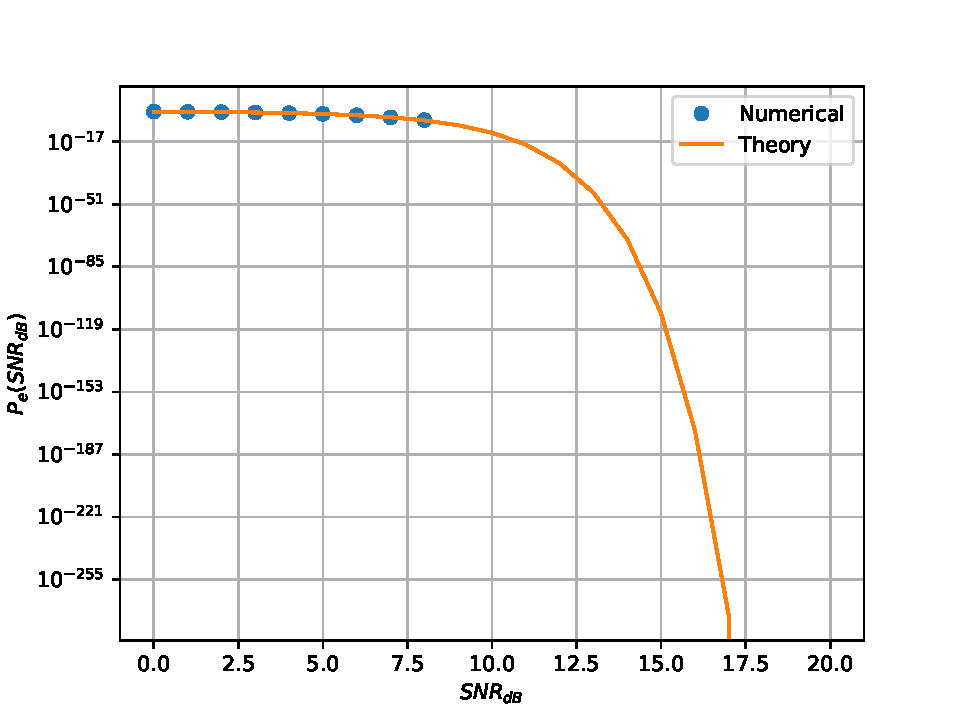
\includegraphics[scale=0.8]{chapter5/figs/biv_pe_vs_snr.pdf}
\caption{$P_e$ with respect to the SNR from 0 to 10 dB}
\label{fig:biv_pe_snr}
\end{figure}
%
\end{enumerate}
